\documentclass[twocolumn]{aastex631}

\usepackage{graphicx}
\usepackage[caption=false]{subfig}
\usepackage{amsmath}
\usepackage{lipsum}
\usepackage[]{mdframed}
\usepackage{booktabs}

\usepackage{newtxsf}

\shorttitle{Autodiff for 2D echellograms}
\shortauthors{Gully-Santiago}

\begin{document}
\title{Towards a Spectrograph Digital Twin: Forward Modeling Pixels of 2D \'Echellograms with Interpretable Machine Learning}

\author{Michael Gully-Santiago}
\affiliation{University of Texas at Austin Department of Astronomy}

\author{TBD}
\affiliation{TBD}


\begin{abstract}

  We introduce autodiff for 2D echellogram forward modeling.

\end{abstract}

\keywords{data: data analysis ---  stars: statistics}


\section{Introduction}\label{sec:intro}

Virtually all modern insights derived from observational optical and near-infrared spectroscopy first arrive through the lossy, imperfect, and unavoidable process of digitization onto a 2-dimensional (2D) focal plane array detector.  Moore's law has propelled the amount of spectrosopic information we can cram onto these detectors over the last 50 years, with the number of pixels catapulting up to a billion-fold.  Innovative optical designs have made evermore effective use of these pixels with information-rich multi-object, imager slicer, and \`echellogram spectral formats.  The computerized distillation of these spectrograms is generally turnkey.  Facility reduction pipelines provide the humdrum ``extraction'' of raw 2D pixels to familiar 1D extracted spectra, ideally an afterhought in a practioner's journey from observation to scientific results.

But increasingly our greatest scientific ambitions are pushing against the limits of how much information we can squeeze out of a given spectrographic observation.  The discovery of other Earths, the redshift of the epoch of reionization, and some of the most important unrealized astronomical discoveries in a generation will occur in the margins of what our most powerful spectrographs can deliver.

The measurement of Extreme Precision Radial Velocity (EPRV) stands out as particularly susceptible to the vagueries of the spectral extraction process.  The instrumental Radial Velocity (RV) precision needed to detect an Earth-like planet around a Sun-like star amounts to $<10$ cm/s, equivalent to a distance of 10 silicon atoms in a typical spectrograph pixel \citep{2014SPIE.9147E..1GM}.  Sub-pixel flat field variations \citep{2018SPIE10698E..5JV}, charge transfer inefficiencies \citep{2020SPIE11454E..0SA}, and other seemingly pathological materials science phenomena matter at these precisions.  Spectral extraction is \emph{not} turnkey at the level of 10 Si atoms.  These precision demands have catalyzed a renewed interest in understanding the delicate interplay of the incident stellar spectrum with the detector pixels.

Most 2D \'echellogram data reduction pipelines can be described as data-driven extraction procedures as opposed to interpretable scene models. The most auspicious of these procedures may be ``Optimal Extraction'' \citep{1986PASP...98..609H}, which treats each column as an independent example of a 1D line profile, enabling a judicious weighting in the cross-dispersion direction.  This prescription faithfully incorporates low-but-significant Signal-to-Noise Ratio (SNR) pixels.  Translating Optimal Extraction to \'echelle spectra gets complicated by the dense and sometime overlapping layouts of the so-called \'echellogram format.  Spectral traces generally do not align with the pixel coordinates, often curving into smile-shaped arcs.  Specialized methods have been developed to handle such layouts \citep{2002A&A...385.1095P,2014A&A...561A..59Z,2020arXiv200805827P}.

The desire to reach the elusive photon-noise limit motivated a subtle mental leap compared to Optimal Extraction.  \emph{Spectroperfectionism} \citep{2010PASP..122..248B} represents a \emph{scene model}, allowing 2D PSF shapes with possibly asymmetric morphologies, convolved with an underlying super-resolution 1D spectrum with unknown spectral structure.  This 2D PSF better resembles the aberrations of a genuine optical system, albeit with the downsides of high computational cost and the inevitability of introducing artificial ringing artifacts into the deconvolved spectrum\footnote{\url{https://hoggresearch.blogspot.com/2019/10/complexifying-optimal-extraction.html}}.  The spectroperfectionism approach has recently been demonstrated on \'echelle spectra for PRV purposes, achieving comparable performance as optimal extraction for the MINERVA spectrograph \citep{2019PASP..131l4503C}, a promising advance towards EPRV.

These existing techniques generally suit the vast majority of use cases, but necessarily cannot handle all science applications.  For example, spatially resolved binaries with separations less than the spectrograph slit length can be acquired with alignment along a spectrograph entrance slit, nominally offering two spectra for the price of one.  But data acquired in this non-standard manner would break most normal pipelines.  More generally, any extended source, such as a photo-dissociation regions (PDR), Solar System planet surfaces, or resolved circumstellar Keplerian gas disks, possess an admixture of spatial and spectral information convolved together in a way that can make separation and interpretation difficult.  A hypothetical general-purpose spectroscopic scene model would be enormously helpful in these contexts, but few such plug-and-play solutions exist.  Spectroastrometry \citep{2011ApJ...733...84P} and the recent slitless scene model for CTIO \citep{2023arXiv230704898N} stand out as recent successes.

Brown dwarfs represent a particularly adversarial example for spectral extraction for two reasons.  Their intrinsically low luminosities mean that all but the closest brown dwarfs have low signal-to-noise ratio at high spectral resolution with existing facilities.  Their ultracool atmospheres contain many molecular absorption bands, in which large swaths of spectra plunge to near zero detectable flux.  The combination of low signal-to-noise ratio and large chunks of missing continuum means that the mere act of identifying a spectral trace becomes difficult, breaking core assumptions in Optimal Extraction.  An even more extreme example---emission line sources---lack a continuum entirely, defying the common pipeline assumption that some detectable signal resides in each pixel sequence.  Heuristics for handling these special cases may exist, but they are often bespoke or require user intervention to guide the process along.

\begin{figure*}[t!]
  \centering
  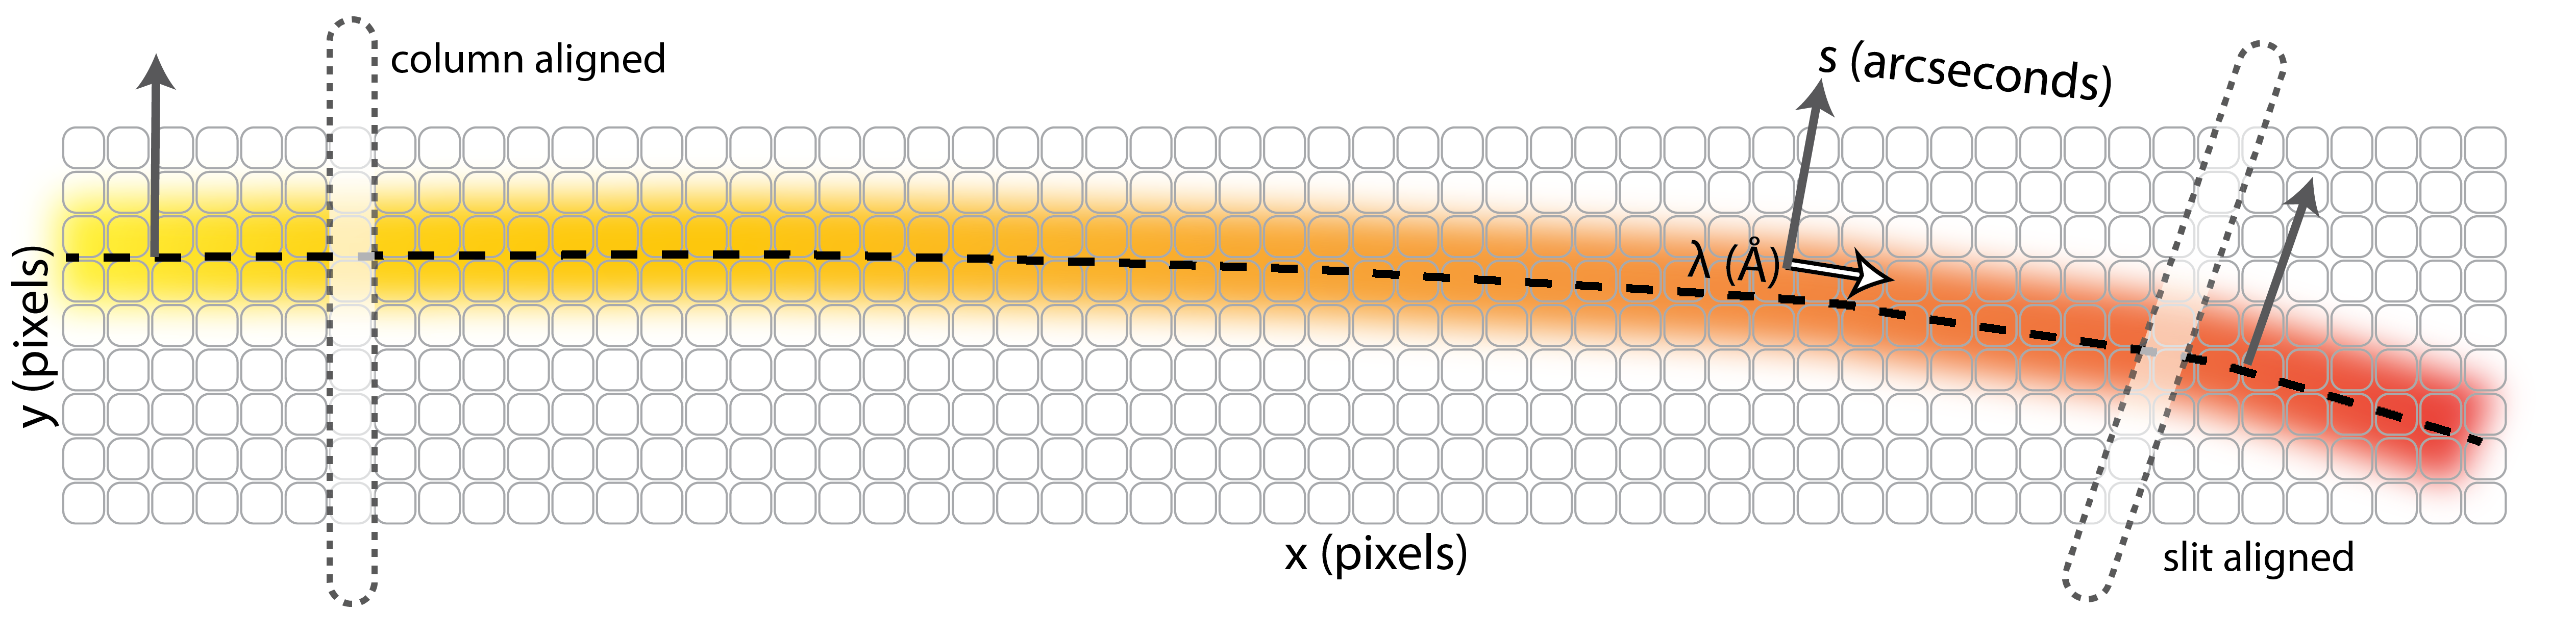
\includegraphics[width=0.98\linewidth]{figures/spectral_trace_v0p1rot.png}
  \caption{Spectral trace geometry for curved \'echellograms.  A spectral trace that has the dispersion axis $\hat{\boldsymbol{\lambda}}$ perfectly aligned with the pixel $\hat{\boldsymbol{x}}$ row vector (``column aligned'') can safely undergo ``optimal extraction'' \citep{1986PASP...98..609H}.  But as the trace curves, the cross-dispersion axis $\hat{\boldsymbol{s}}$ tilts away from the verical columns $\hat{\boldsymbol{y}}$.  An ideal extraction box may be aligned with the cross-dispersion axis (``slit aligned'' for a slit-based instrument).  The right choice for extraction becomes complicated in this scenario and forms the basis of this paper.}
  \label{fig:traceSchematic}
\end{figure*}


Even in EPRV, the assumptions in optimal extraction are not actually optimal, and the choices in spectroperfectionism not actually perfect.  Optimal extraction generally treats the cross-dispersion direction as exactly aligned with the detector $y$ axis as illustrated in Figure \ref{fig:traceSchematic}. This computationally expedient heuristic could be expected to introduce small RV biases that grow as the spectral traces tilt and bend farther from the detector pixel alignment.  As seen in the right side of Figure \ref{fig:traceSchematic}, the cross-dispersion axis (normal to the dispersion direction), tilts away from the columns. Straight-line tilted traces have the effect of polluting adjacent wavelength bins in nearly equal measure and, to first order, lowering the effective spectral resolving power.  Ideally we would extract along the cross-dispersion axis (``slit-aligned''), but doing so may force us to re-grid the spectrum via intepolation, a loss mechanism that loses the native pixel uncertainties by correlating adjacent pixels.

Curved \'echelle traces are even more insidious.  The smearing of pixels can be expected to proceed with a systematic RV shift, since the shoulder of one spectral line notices slightly more of its pixel neighbor to the left or right, depending on the extent and direction of the spectral trace's curvature.  These seemingly pathological minor biases must make a difference at the 10 Si atom level, but quantifying such complex effects has been elusive in part due to the lack of an end-to-end simulation framework for \'echellograms.

We seek a spectrograph's \emph{digital twin}.  This term refers to a class of extreme forward modeling--a digital twin should represent all or most of the relevant behaviors of a complex system in a way that can be interrogated to build novel insights.  A digital twin should resemble---as close as possible---the actual state of the system at any given moment, providing simulated data that is indistinguishable from a genuine observation.  An \'echelle spectrograph digital twin therefore builds upon and transcends the notions of scene modeling introduced in \citet{2010PASP..122..248B}, by aspiring to include evermore realistic attributes of the spectrograph's imaging system into the computational machinery.  A digital twin would improve upon these limitations by providing a more physically realistic generative model for the underlying spectrum.

The challenges of creating a spectrograph's digital twin are enormous.  Generally only a few individual practitioners possesses the requisite knowledge of all the copious ways a spectrograph may be perturbed, and an even smaller fraction of such individuals have the capacity or desire to translate those perturbations into an evaluable forward scene model.  Even if such a model could be written down and codified into a program, evaluating that program is destined to be computationally expensive owing to a litany of \texttt{for} loops on millions of pixel-based simulations.  Any likelihood function would need to be re\"evaluated as a Bayesian inverse problem to determine the settings of the tunable scene model.  The spectrograph state, sky emission lines, and underlying target star spectrum may have tens of thousands of variables needed to adequately describe the spectrogram.  Tuning tens of thousands of non-linear parameters in this complicated forward model would appear hopelessly intractable.  Even if one could somehow linearize a large subset of these parameters via linear algebra \citep{2010PASP..122..248B}, correlated residual structures would inevitably predominate the likelihood calculation, hampering the application of computationally expedient chi-squared algorithms.

Machine learning innovations make digital twins newly possible. First, and most importantly, machine learning frameworks such as PyTorch \citep{2019arXiv191201703P}, Tensorflow \citep{tensorflow2015-whitepaper}, and JAX \citep{jax2018github} offer end-to-end atomatic differentiation.  This key enabling technology makes it possible to tune an unlimited number of non-linear parameters through the process of vectorized Stochastic Gradient Descent \citep[SGD,][]{2016arXiv160904747R}, or simply \emph{backprop}.  Second, these frameworks all offer seamless integration with hardware accelerators, including Graphical Processing Units (GPUs) and Tensor Processing Units (TPUs), that can yield 60-100$\times$ speedups with no code change.  Third, neural network architectures and/or kernel methods offer a strategy for learning patterns in correlated residual structures, which has the effect of making likelihood functions tolerant to inevitable imperfections in the forward model.  All together these and other modern computational innovations unlock a truly new category of ambition for our data analysis, bringing a full spectrograph forward model into reach.

In this work, we introduce a new interpretable machine learning framework for the analysis of 2D \'echellograms.  We write down and illustrate the the design of the forward model in \S \ref{secMethod}, including a breakdown into sky, target, and background steps.  These steps are generally agnostic to the spectrograph design, and could apply to either a slit-based or fiber-fed instrument with some tuning.  We choose to design our protoype on archival Keck NIRSPEC spectra of faint ultracool brown dwarf spectra, a category already identified as particularly vulnerable to poor optimal extraction.  In \S \ref{results1Synthetic}, we first illustrate the injection and recovery of known signals in synthetic spectrograms, running the synthetic spectra through facility pipelines as if they were bona fide observations.  We then show the results on genuine data in \S \ref{results1Synthetic}, comparing the end-to-end performance of our technique with facility pipelines.  Finally in \S \ref{secDiscuss}, we discuss the tradeoffs of the technique and ways in which it could be extended, and design considerations for other applications.  We discuss economic considerations of applying the framework, weighing the computational cost against the lifecycle cost of traditional spectral acquisition and analysis.  Throughout the work we dispell common criticisms of machine learning as a black box, since our method surgically adopts the interpretable components of the multi-faceted technology while largely eschewing fashionable-albeit-uninterpretable neural network architectures.  We provide the Python implementation as an open source code, \texttt{ynot}\footnote{\url{https://github.com/gully/ynot}}.  We intend the framework to serve as community destination for modular experimentation on digital twins for astronomical spectroscopy.


\section{Methodology: Modeling 2D Pixels} \label{secMethod}

\subsection{Autodiff as a central design choice}
Our method has one uncompromising architectural decision that drives many subsequent design features: we must have automatic differentiation.  Without \emph{autodiff}, the optimization of our spectrogram scene model would be intractable.  The need for autodiff restricts our adoption of programming language to only one of three or four popular Machine Learning (ML) frameworks, since these ML frameworks offer autodiff by construction.  Which of these several ML frameworks to select is a matter of taste--we implemented our method in \texttt{PyTorch}, and anticipate a future prototype may be written in \texttt{JAX}.  Both of these provide partial derivatives of the likelihood function $\mathcal{L}$ with respect to all input parameters of the scene model:

\begin{equation}
  \frac{\partial{\mathcal{L}}}{\partial{\vec{\theta}}} \label{eq1}
\end{equation}

\noindent where $\vec{\theta}$ represents the vector of tunable parameters that we will soon encounter, and will occupy the lion's share of this section.  We anticipate the length of $\vec{\theta}$ to number in the tens of thousands of parameters.  Models that can provide Equation \ref{eq1} are called \emph{differentiable}.  One consequence of requiring our models to be differentiable is that we cannot use any outside libraries: \texttt{astropy}, \texttt{Scipy}, and \texttt{numpy} would break the ability of \texttt{PyTorch} to deliver Equation \ref{eq1}.  The constraint to never-leave-\texttt{PyTorch} makes an already difficult task even more difficult, but possible.


\subsection{The Shape of Data and Likelihood}
Data from a raw spectrogram in its purest form contains $d_{ij}$, where $i$ and $j$ are the fixed pixel indices in the $x$ and $y$ directions respectively, and $d$ is the digitized datum value in analog-to-digital units (ADUs).  The full frame image of an \'echellogram is stored as an $(N \times M)$ matrix, which we will call $\boldsymbol{\mathsf{D}}$ to emphasize that this object represents \emph{data}:

\begin{equation}
  \boldsymbol{\mathsf{D}} =  \begin{bmatrix}
    d_{11} & \dots  & d_{1N}                       \\
    \vdots & \ddots & \vdots                       \\
    d_{M1} & \dots  & d_{MN} \label{eqDenseMatrix}
  \end{bmatrix}
\end{equation}

Our digital twin seeks to make an interpretable forward model $\boldsymbol{\mathsf{M}}(\vec{\theta})$ that has the exact same shape as $\boldsymbol{\mathsf{D}}$.  We can then write down the data-model residual matrix and write the familiar $\chi^2$ likelihood function:

\begin{eqnarray}
  \boldsymbol{\mathsf{R}}(\vec{\theta}) = \boldsymbol{\mathsf{D}} - \boldsymbol{\mathsf{M}}(\vec{\theta}) \\
  \mathcal{L} = -\frac{1}{2} \sum_{i=1}^{N}\sum_{j=1}^{M} \left ( \frac{r_{ij}(\vec{\theta})}{\sigma_{ij}} \right )^2 \label{eqChiSq}
\end{eqnarray}

where the $\sigma_{ij}$ are the nominally fixed per-pixel uncertainty estimates.  Written in this way, we can see that every pixel can---at least in principle---inform every model parameter.  Equation \ref{eq1} senses what infinitesimal changes to each model parameter would result in a closer match to the data, a higher likelihood $\mathcal{L}$ (\emph{i.e.} a lower $\chi^2$).  This statement encodes the hope of a digital twin, that by leveraging all of the raw data, our constraints on the state of the spectrograph can be as well-informed as possible.

\subsection{Cartesian pixels to spectrum-centric coordinates}



The chief operation of a spectrograph is to disperse overlapping light into different spatial coordinates.  Spectral extraction aims to \emph{undo} that process, seeking a lookup table of $x$ coordinates to wavelength coordinates $\lambda$.  Here we introduce the 2D analog of wavelength calibration, seeking a mapping from $(x, y)$ pixels to some as-yet-unspecified spectrograph-centric coordinate system.  Spectrograms encode two unseen native spectral coordinates, the dispersion axis $\lambda$ and the cross-dispersion axis that we will designate as $s$.  Diffractive optical elements such as \'echelle gratings have an additional special property of repeating spectral coordinates into adjacent \'echelle orders, indexed as $m$, according to the grating equation \citep{2012sdf..book.....J}.  The mapping of the physics-based coordinates $(\lambda, s, m)$ to the detector $(x, y)$ Cartesian pixel coordinate system can be abstracted as some enormously complicated continuous vector-valued function $G$:

\begin{equation}
  G(x,y) = (\lambda, s, m)
\end{equation}

Nature does not know about $G$, but instead its similarly complicated inverse: $G^{-1}(\lambda, s, m) = (x,y)$.  The choice of how to obtain $G$ (or its inverse) forms our second key architectural design consideration (after requiring autodiff).  Hypothetically, $G$ could be derived from the spectrograph's optical design software, validated with in-lab optical metrology, and adjusted for on-sky performance. Common software already takes $(\lambda, s, m)$ as inputs and returns focal plane coordinates as outputs, so this physically-motivated $G^{-1}$ appears ideal for a digital twin. But optical modeling comes with some challenges and tradeoffs.  First, most optical designs are conducted in a proprietary program such as Zemax\texttrademark, which is generally incompatible with Eq. \ref{eq1}: you cannot take partial derivatives of a Zemax model.  An suitable alternative could be to rewrite your entire optical model in a differentiable optical modeling framework such as \texttt{morphine} \citep{2021ApJ...907...40P} or $\partial{\mathrm{Lux}}$ (Desdoigts et al. \emph{in prep}).

For now, we simply treat $G$ as a phenomenological parametric model, and emphasize that the \texttt{ynot} code is written in a future-proof way, such that the $G$ module can be hot-swapped with a drop-in-replacement physics-based model if/when one becomes available.


\subsection{Breaking the scene into local and global components}
In practice, not all pixels inform all parameters.  So our third key architectural design choice is to separate physical and instrumental effects as being either global or local.  Local physical or instrumental effects are much easier to model than global ones, since their computation can be restricted to a subset of all pixels.  We identify a science target frame as consisting of 5 distinct constituent layers, only some of which touch all pixels.  For example, all pixels exhibit a distinct global bias and thermal background response: a changing detector temperature generally affects all pixels.  Conversely, only some pixels ``see'' the sky background, and an even smaller subset sense the thin trace of the science target spectrum.  Scattered light and/or internal optical reflections are somewhere in-between, depending on the scale-length and angles of scattering.  Additional binary layers for dead pixels and cosmic ray masks can be treated similarly, for a total of 7 distinct physical or instrumental layers that may affect any given pixel.  The model can be re-written as some separable combination of these constituent parts, and in the process we can designate the native coordinate system of each component:

\begin{equation}
  \begin{split}
    \boldsymbol{\mathsf{M}}(\vec{\theta}) = \; &\boldsymbol{\mathsf{M}}_{\mathrm{b}}(x,y) \quad \textcolor{lightgray}{\text{\emph{bias term}}}\\
    + \;&\boldsymbol{\mathsf{M}}_{\mathrm{t}}(x,y) \quad \textcolor{lightgray}{\text{\emph{thermal response}}}\\
    + \;&\mathsf{M}_\mathrm{sky}(\lambda, s, m) \quad \textcolor{lightgray}{\text{\emph{sky emission}}}\\
    + \;&\mathsf{M}_\mathrm{targ}(\lambda, s, m) \quad \textcolor{lightgray}{\text{\emph{science target}}}\\
    + \;&\textcolor{gray}{\texttt{[scattered light term]}} \\
    + \;&\dots \quad \textcolor{lightgray}{\text{\emph{miscellaneous}}}
  \end{split}
\end{equation}

The bias and thermal response (\emph{i.e.} dark) terms depend chiefly on the state of the spectrograph's readout electronics and detector temperature, and are usually considered fixed and determined \emph{a-priori}.  Our spectrograph's digital twin forward scene model will allow these terms to take on a parameteric form described in Appendix \ref{secAppendixDataTypes}, amounting to a relatively negligible effect for most applications.  We ignore the scattered light term and other miscellaneous terms for now as well, a fair assumption for many spectrographs and use cases.

The sky emission and target terms are special.  First, they reside in spectrograph coordinates, which can be converted to spatial pixels with $G^{-1}$.  Second---as emphasized above---their reach is local.  We therefore adopt \emph{sparse matrices} to represent the sky and science target terms. We assign the slightly nonstandard convention of denoting sparse matrices with the un-bolded symbol $\mathsf{M}$, and their counterpart \emph{dense matrices} with the bold version.  A sparse matrix can be pictured as resembling a vector, since it stores only the non-zero elements as a trio of coordinates-and-value, and assumes zeros for all other entries.  We can visualize an example sparse matrix as an augmentation to Equation \ref{eqDenseMatrix}:

\begin{equation}
  \mathsf{M} =  \begin{bmatrix}
    (7, 2, m_{72}) \\
    \vdots         \\
    (i, j, m_{ij}) \\
    \vdots         \\
    (3, 5, m_{35})    \label{eqSparseMatrix}
  \end{bmatrix}
\end{equation}

\section{How to represent the target spectrum}

\begin{figure*}[t!]
  \centering
  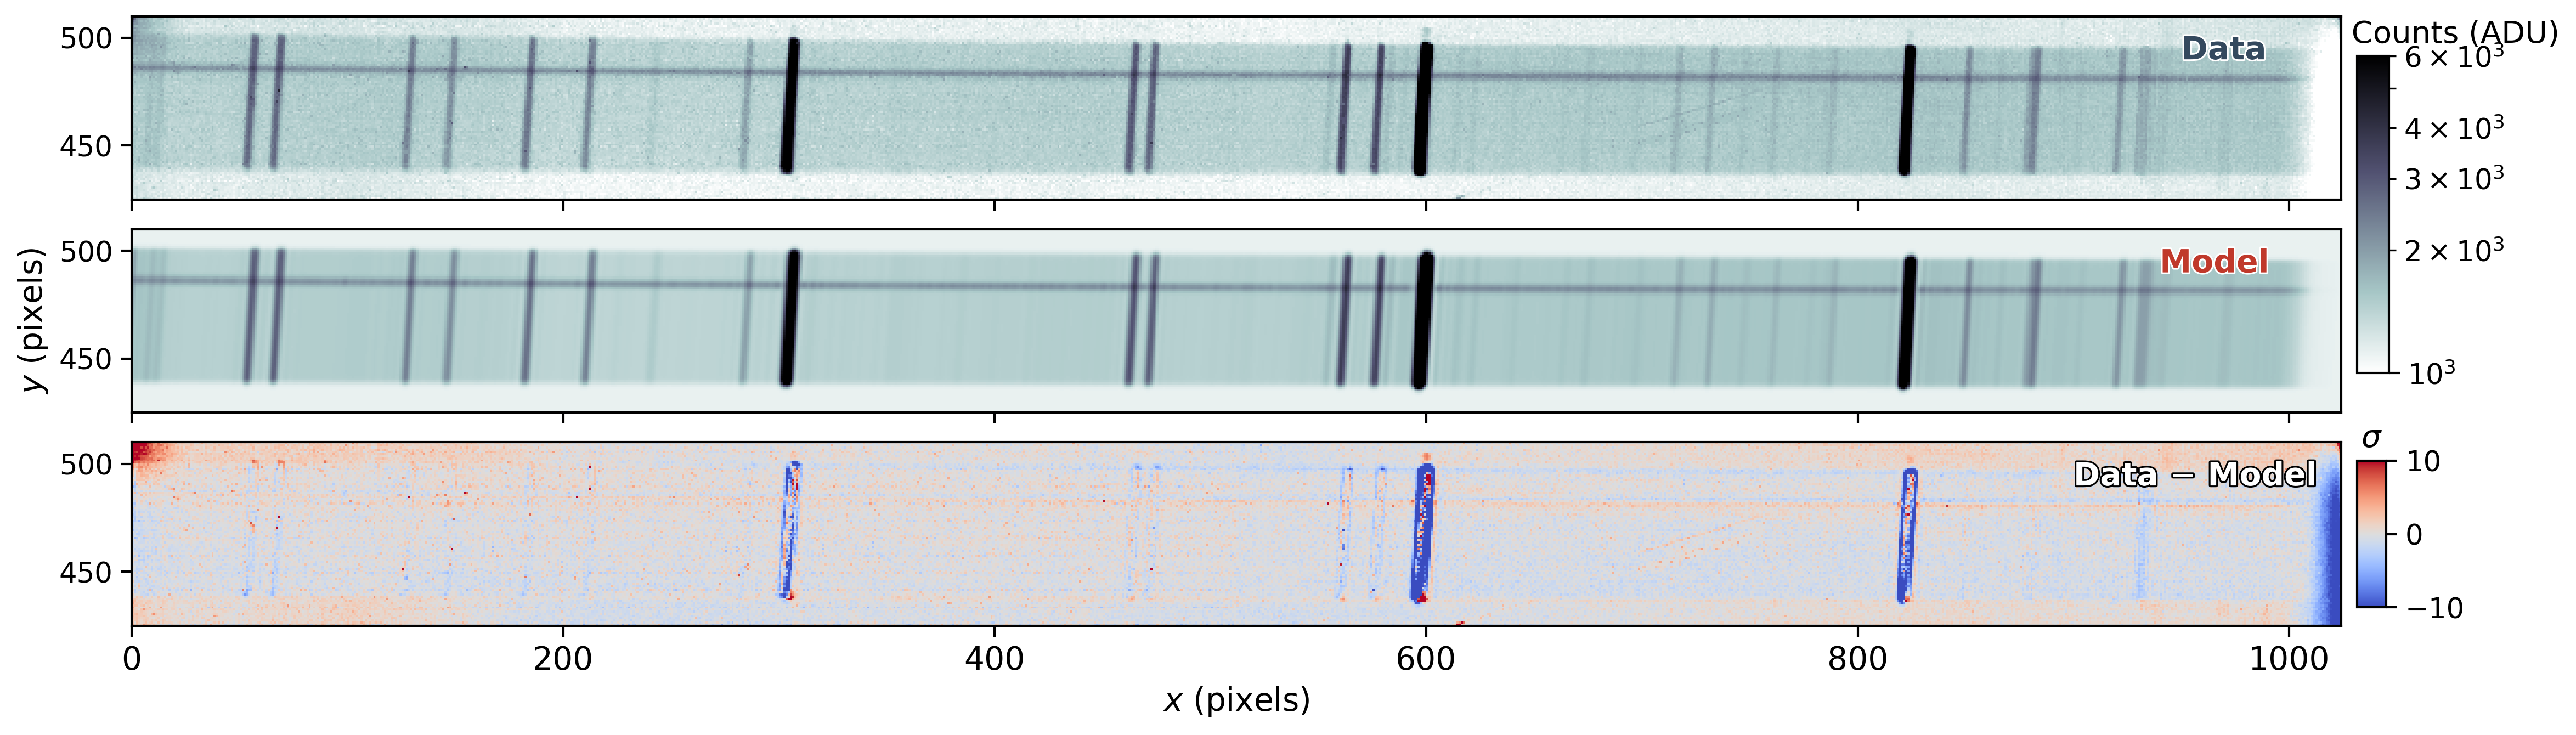
\includegraphics[width=0.98\linewidth]{figures/scene_model_single_order.png}
  \caption{Scene model for a portion of a Keck NIRSPEC \'echellogram centered on a single spectral order.  The sky lines, \'echelle order boundaries, and stellar point source spectral trace appear as familiar features.  Skyline emission lines exhibit the greatest residual amplitudes.  The residual also exhibits minor structures near the photon noise limit, such as detector pattern noise.  Vignetting can be seen at the right edge and upper left corner.}
  \label{fig:sceneModelSingleOrder}
\end{figure*}

Writing down a model for the science target spectrum represents both the chief science objective, and nearly circular reasoning. We need to know the underlying spectrum of the target star in order to fully model the scene, but if we had perfect knowledge of the target star we would not need to model the scene, nor take any data in the first place.  Instead we have to infer the spectrum.  The right choice depends strongly on one's science goals, and there does not exist a single best choice for all use cases.  Here we narrate three pathways.

We could simply have a non-parameteric super-resolution highly flexible model for the underlying spectrum that gets iteratively updated and solved for.  This strategy works adequately \citep{2010PASP..122..248B}.

Relatedly, we could employ a differentiable tunable model, such as \texttt{wobble} \citep{2019AJ....158..164B} or \emph{blas\'e} \citep{2022ApJ...941..200G}.

Finally, if the end-goal of the science analysis is to fit a tunable model to the spectrum, the data-model comparison could simply take place directly in the 2D \'echellogram pixels, instead of ever acquiring the 1D extracted spectrum as an intermediate data product.

We choose a combination of the first two options, most resembling a crossover of  \citet{2010PASP..122..248B} to \citet{2019AJ....158..164B}.  For the rest of the paper we will simply assume the target is a stellar point source, though the technique is relatively agnostic to the astrophysics of the source properties.  We write down the parameterized stellar spectrum as a contiguous string of adjacent and overlapping 2D Gaussians, each located at wavelength coordinate $\lambda_k$.

\begin{equation}
  f_k(\lambda_k) = A_k e^{-\left (\frac{\lambda - \lambda_k}{\epsilon} \right )^2}
\end{equation}


\begin{mdframed}
  \textbf{How to represent the target spectrum} \par
  - How to represent the sky spectrum\par
  - How to represent the target PSF\par
  - How to represent the sky spatial extent\par
  - How to represent the slit\par
\end{mdframed}


\subsection{Constructing a Resilient Likelihood}
\begin{mdframed}
  \textbf{The need to joint model, regularize, address outliers} \par
  - The likelihood function and per-pixel uncertainties\par
  - Arcs: sparsely encode both wavelength and slit position\par
  - Flats: encode just slit position\par
  - Darks: encode just background\par
  - Target spectra: encode wavelength, slit position, target position\par
  \textcolor{lightgray}{\lipsum[7]}
\end{mdframed}


\section{Results 1: Training on Synthetic Data with Injection/Recovery Tests} \label{results1Synthetic}

\begin{mdframed}
  \textbf{Injection/recovery test with noisy data: generating fake data} \par
  \textcolor{lightgray}{\lipsum[9]}
\end{mdframed}

\begin{mdframed}
  \textbf{Initializing of the model and optimization setup} \par
  \textcolor{lightgray}{\lipsum[10]}
\end{mdframed}


\begin{mdframed}
  \textbf{Training computational performance} \par
  - Number of epochs\par
  - Batching/sparsity\par
  \textcolor{lightgray}{\lipsum[9]}
\end{mdframed}

\begin{mdframed}
  \textbf{Best fit model comparison 1: injection/recovery of initial parameters} \par
  - Number of epochs\par
  - Batching/sparsity\par
  \textcolor{lightgray}{\lipsum[10]}
\end{mdframed}

\begin{mdframed}
  \textbf{Best fit model comparison 2: spectrum as unbinned, weighted samples} \par
  - Number of epochs\par
  - Batching/sparsity\par
  \textcolor{lightgray}{\lipsum[11]}
\end{mdframed}


\section{Results 2: Training on real data}
\begin{mdframed}
  \textbf{Introduction to real data} \par
  - Data-preprocessing and heuristics \par
  \textcolor{lightgray}{\lipsum[12]}
\end{mdframed}

\begin{mdframed}
  \textbf{Outcome: reduced spectrum as unbinned, weighted samples} \par
  - SNR improvement compared to previous methods (head-to-head)\par
  \textcolor{lightgray}{\lipsum[13]}
\end{mdframed}

\pagebreak
\clearpage

\section{Discussion}\label{secDiscuss}

\begin{mdframed}
  \textbf{Philosphy: Each previous spectrum should inform future spectra} \par
  Treat the instrument as a breathing, dynamic system\par
  \textcolor{lightgray}{\lipsum[5]}
\end{mdframed}

\begin{mdframed}
  \textbf{The promise for EPRV} \par
  - Simulation of minor RV shifts\par
  - Simulation of sub-pixel flat fields \par
  - Tracking spectrograph state across decades of operation\par
  \textcolor{lightgray}{\lipsum[14]}
\end{mdframed}


\begin{mdframed}
  \textbf{Ability to repurpose non-standard data (variable data quality)} \par
  \textcolor{lightgray}{\lipsum[15]}
\end{mdframed}


\begin{mdframed}
  \textbf{Conceivable extensions} \par
  \textcolor{lightgray}{\lipsum[16]}
\end{mdframed}



\begin{acknowledgements}
  %% May also acknowledge XRP and TESS: 
  % 80NSSC20K0257 for the XRP program, and 80NSSC22K0181 through the TESS Guest Investigator program 
  This material is based upon work supported by the National Aeronautics and Space Administration under Grant Number 80NSSC21K0650 for the ADAP program issued through the Science Mission Directorate.

  C.V.M. acknowledges support from the Alfred P. Sloan Foundation under grant number FG-2021-16592.

  This research has made use of the Keck Observatory Archive (KOA), which is operated by the W. M. Keck Observatory and the NASA Exoplanet Science Institute (NExScI), under contract with the National Aeronautics and Space Administration.

  This research has made use of NASA's Astrophysics Data System.
\end{acknowledgements}


\facilities{Keck (NIRSPEC), Gaia}

\software{  pandas \citep{mckinney10, reback2020pandas},
  matplotlib \citep{hunter07},
  numpy \citep{harris2020array},
  scipy \citep{jones01},
  ipython \citep{perez07},
  pytorch \citep{NEURIPS2019_9015}}

\appendix

\section{Comparison to other frameworks}

Hundreds or possibly thousands of 2D extraction pipelines have been written and rewritten to suit the disparate needs of each unique spectrograph.  Table 1 of \citet{2022PASP..134k4509C} lists 18 \'echelle spectrographs and their data reduction pipelines.  Many but not all of those pipelines are open source.  Here we list a subset of recent open source pipelines for \'echelle spectra reduction.

Few approaches have attempted to combine spectral scene modeling in combination with machine learning techniques.  \citet{2020MNRAS.499.1972X} employed a 2D PSF convolution with neural networks on a demonstration with multi-object spectra from LAMOST.  While promising, the code is not open source and the applications limited to inferring the field distortion, but not extending to subsequent extraction steps.

\citet{2019PASP..131l4503C} developed spectroperfectionism for the MINERVA spectrograph, finding similar performance as optimal extraction.


\begin{deluxetable*}{lllll}
  \tablewidth{0pc}
  \tablecaption{
    Selection of open source codes for 2D echelle data reduction
    \label{tabHeSM}
  }
  \tablehead{
    \colhead{Code}   &
    \colhead{Instrument} &
    \colhead{Reference} &
    \colhead{Language} &
    \colhead{Note}
  }
  \startdata
  \hline
  \multicolumn{5}{c}{\'echelle} \\
  \hline
  \href{https://github.com/igrins/plp}{PLP} & IGRINS & \citet{2014AdSpR..53.1647S, jaejoonlee15} & Python & \\
  \href{https://github.com/AWehrhahn/PyReduce}{PyReduce} & HARPS, UVES & \citet{2021AA...646A..32P} & Python & \\
  \href{https://github.com/njcuk9999/apero-drs}{APERO} & SPIRou & \citet{2022PASP..134k4509C} & Python &\\
  \hline
  \multicolumn{5}{c}{Long-slit} \\
  \hline
  \href{https://github.com/LSSTDESC/Spectractor}{Spectractor} & CTIO & \citet{2023arXiv230704898N} & Python & Scene Modeling\\
  \enddata
  \tablecomments{Some codes are applicable to multiple instruments, and some instruments have multiple codes.}
\end{deluxetable*}

\section{Flat fields, Dark, and Arc Frames} \label{secAppendixDataTypes}

Every spectrograph is different, but several common categories of raw data frames can be expected: flat field frames $\boldsymbol{\mathsf{D}}_{\mathrm{flat}}$, dark frames $\boldsymbol{\mathsf{D}}_{\mathrm{dark}}$, wavelength calibration frames $\boldsymbol{\mathsf{D}}_{\mathrm{arc}}$, and science target frames $\boldsymbol{\mathsf{D}}_{\mathrm{targ}}$.  For our purposes, observations of standard-star frames reside in the science target frame category, since they share the same observational configuration.  Most of the main text of this document focused on the modeling of the science target frame, and so we simply dropped any subscripts and referred to this auspicious data as simply $\boldsymbol{\mathsf{D}}$.  All of these calibration frames inform the state of the spectrograph, and can and should be used as such.  The \texttt{ynot} framework provides specialized modeling for these datatypes.

\clearpage

\bibliography{ms}

\end{document}
